\documentclass{article}
\usepackage{tikz}

\begin{document}

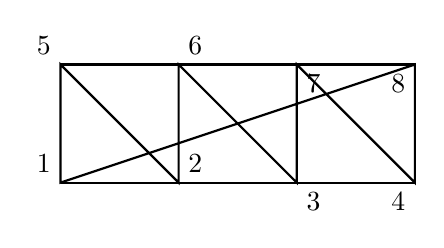
\begin{tikzpicture}[scale=1.5]
    % Define coordinates for the vertices
    \coordinate (A) at (0,0);
    \coordinate (B) at (1,0);
    \coordinate (C) at (2,0);
    \coordinate (D) at (3,0);
    \coordinate (E) at (0,1);
    \coordinate (F) at (1,1);
    \coordinate (G) at (2,1);
    \coordinate (H) at (3,1);

    % Draw the edges of the graph
    \draw[thick] (A) -- (B) -- (C) -- (D) -- cycle;
    \draw[thick] (E) -- (F) -- (G) -- (H) -- cycle;
    \draw[thick] (A) -- (E) -- (B) -- (F) -- (C) -- (G) -- (D) -- (H) -- cycle;

    % Label the vertices
    \node at (A) [above left] {1};
    \node at (B) [above right] {2};
    \node at (C) [below right] {3};
    \node at (D) [below left] {4};
    \node at (E) [above left] {5};
    \node at (F) [above right] {6};
    \node at (G) [below right] {7};
    \node at (H) [below left] {8};
\end{tikzpicture}

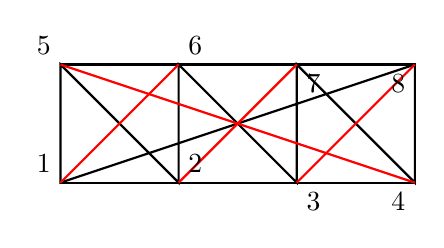
\begin{tikzpicture}[scale=1.5]
    % Define coordinates for the vertices
    \coordinate (A) at (0,0);
    \coordinate (B) at (1,0);
    \coordinate (C) at (2,0);
    \coordinate (D) at (3,0);
    \coordinate (E) at (0,1);
    \coordinate (F) at (1,1);
    \coordinate (G) at (2,1);
    \coordinate (H) at (3,1);

    % Draw the edges of the graph
    \draw[thick] (A) -- (B) -- (C) -- (D) -- cycle;
    \draw[thick] (E) -- (F) -- (G) -- (H) -- cycle;
    \draw[thick] (A) -- (E) -- (B) -- (F) -- (C) -- (G) -- (D) -- (H) -- cycle;
    \draw[red, thick] (A) -- (F);
    \draw[red, thick] (B) -- (G);
    \draw[red, thick] (C) -- (H);
    \draw[red, thick] (D) -- (E);

    % Label the vertices
    \node at (A) [above left] {1};
    \node at (B) [above right] {2};
    \node at (C) [below right] {3};
    \node at (D) [below left] {4};
    \node at (E) [above left] {5};
    \node at (F) [above right] {6};
    \node at (G) [below right] {7};
    \node at (H) [below left] {8};
\end{tikzpicture}

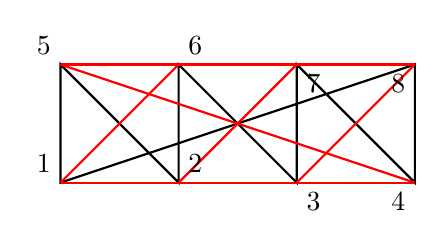
\begin{tikzpicture}[scale=1.5]
    % Define coordinates for the vertices
    \coordinate (A) at (0,0);
    \coordinate (B) at (1,0);
    \coordinate (C) at (2,0);
    \coordinate (D) at (3,0);
    \coordinate (E) at (0,1);
    \coordinate (F) at (1,1);
    \coordinate (G) at (2,1);
    \coordinate (H) at (3,1);

    % Draw the edges of the graph
    \draw[thick] (A) -- (B) -- (C) -- (D) -- cycle;
    \draw[thick] (E) -- (F) -- (G) -- (H) -- cycle;
    \draw[thick] (A) -- (E) -- (B) -- (F) -- (C) -- (G) -- (D) -- (H) -- cycle;
    \draw[red, thick] (A) -- (F);
    \draw[red, thick] (B) -- (G);
    \draw[red, thick] (C) -- (H);
    \draw[red, thick] (D) -- (E);

    % Draw additional edges
    \draw[red, thick] (A) -- (C);
    \draw[red, thick] (B) -- (D);
    \draw[red, thick] (E) -- (G);
    \draw[red, thick] (F) -- (H);

    % Label the vertices
    \node at (A) [above left] {1};
    \node at (B) [above right] {2};
    \node at (C) [below right] {3};
    \node at (D) [below left] {4};
    \node at (E) [above left] {5};
    \node at (F) [above right] {6};
    \node at (G) [below right] {7};
    \node at (H) [below left] {8};
\end{tikzpicture}

\end{document}